\subsection{Construction du troisième parcours différencié en sixième}
\subsubsection*{Évaluation diagnostique}\label{Eval_diag_ju}
\begin{figure}[!h]
	\center{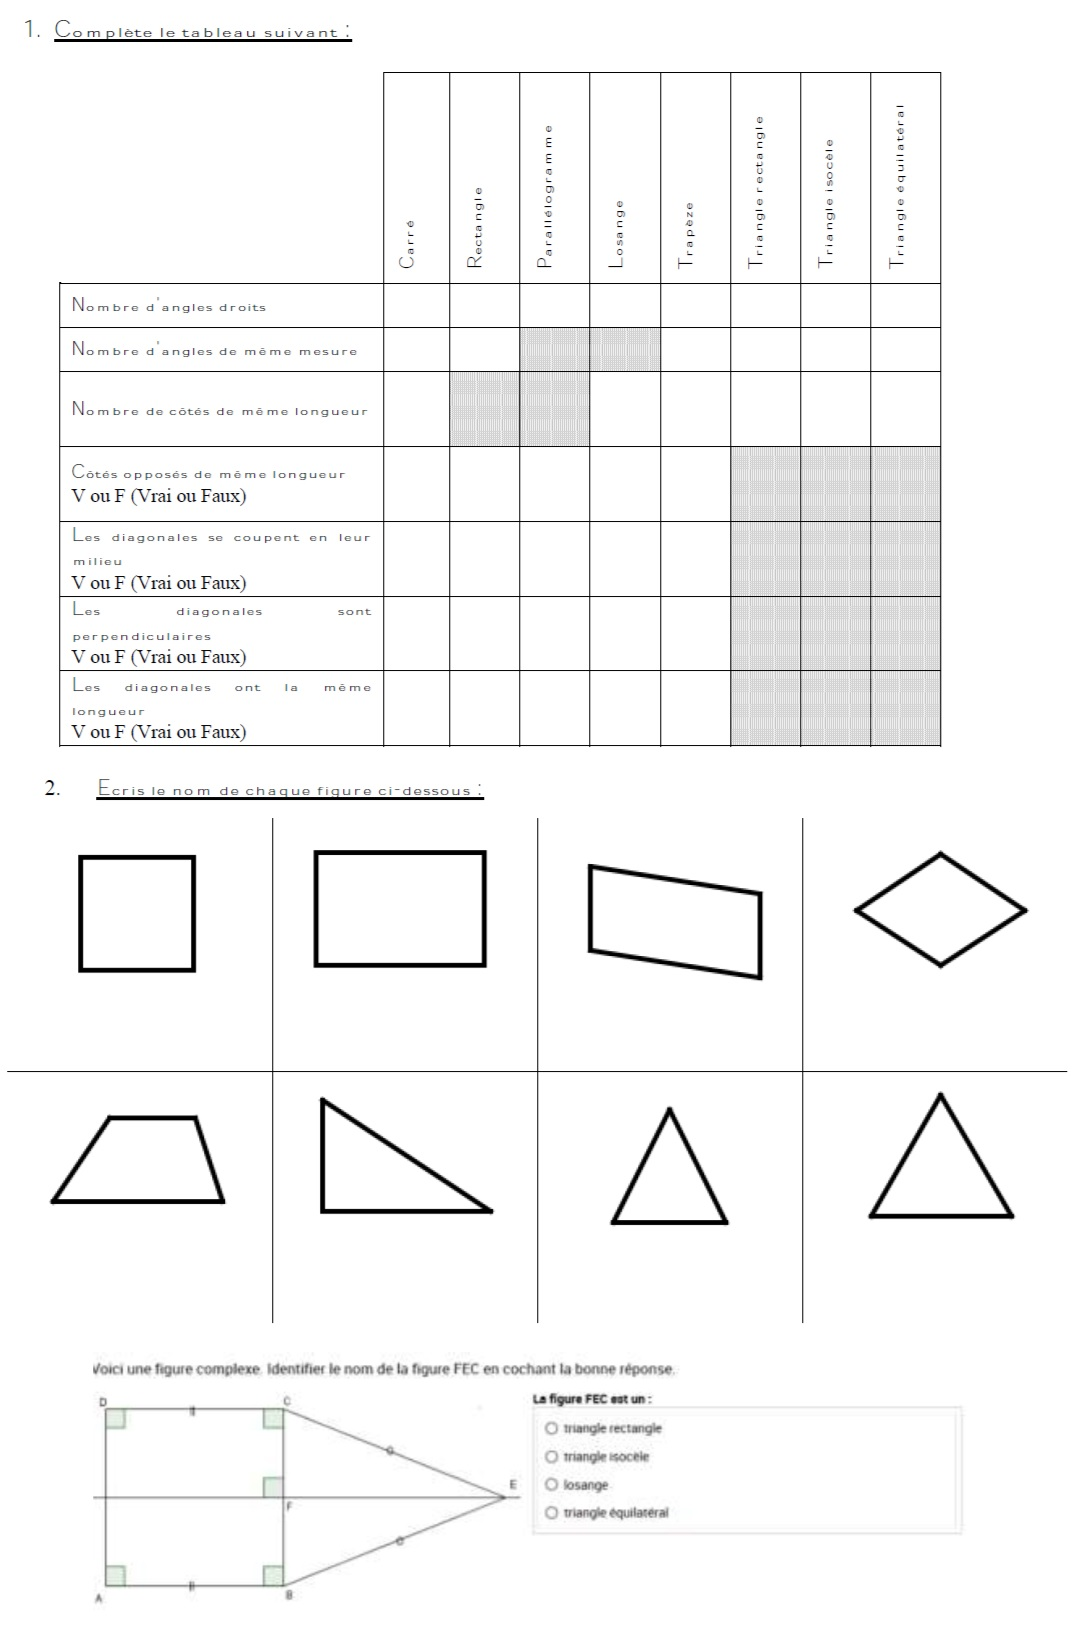
\includegraphics{img/eval_diag_julia.jpg}}
	\caption{Évaluation diagnostique}
\end{figure}
\subsubsection*{Productions d'élèves}
\begin{figure}[!h]
	\centering
	\subfloat[copie n°1]{{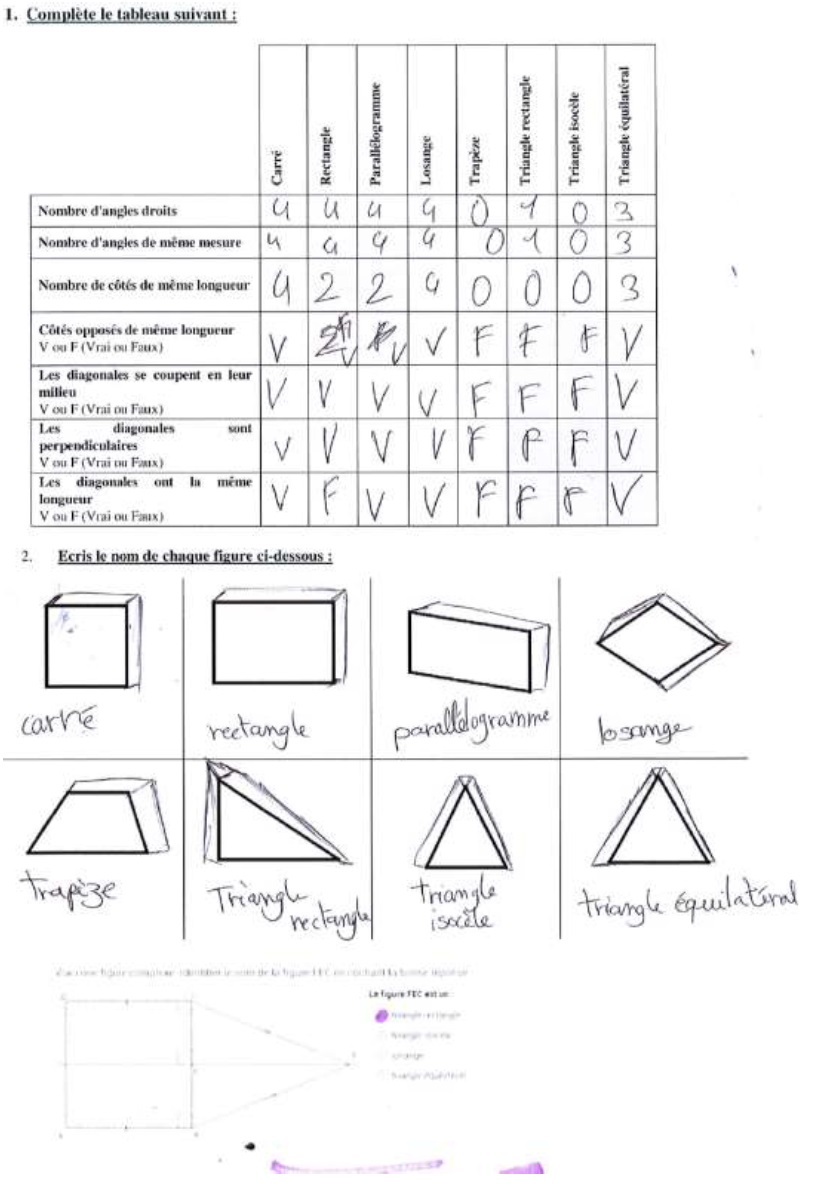
\includegraphics[scale=0.4]{img/copie1_eval_diag_ju.jpg}}}
	\qquad
	\subfloat[copie n°2]{{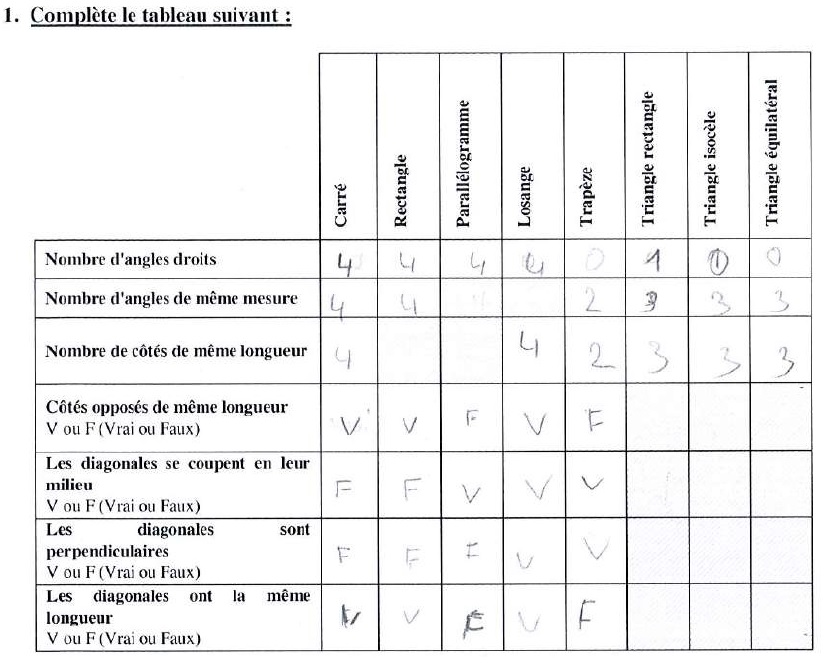
\includegraphics[scale=0.5]{img/copie2_eval_diag_ju.jpg}}}
	\qquad
	\subfloat[copie n°3]{{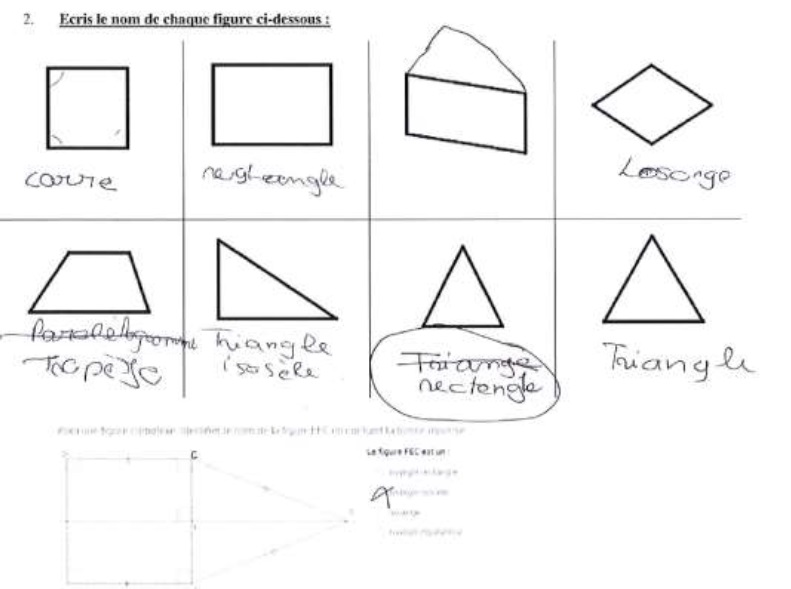
\includegraphics[scale=0.5]{img/copie3_eval_diag_ju.jpg}}}
	\caption{Évaluations d'élèves}
	\label{fig:Eval_diag_copies}
\end{figure}
\subsubsection*{Analyse des productions d'élèves}
\begin{figure}[!h]
	\centering
	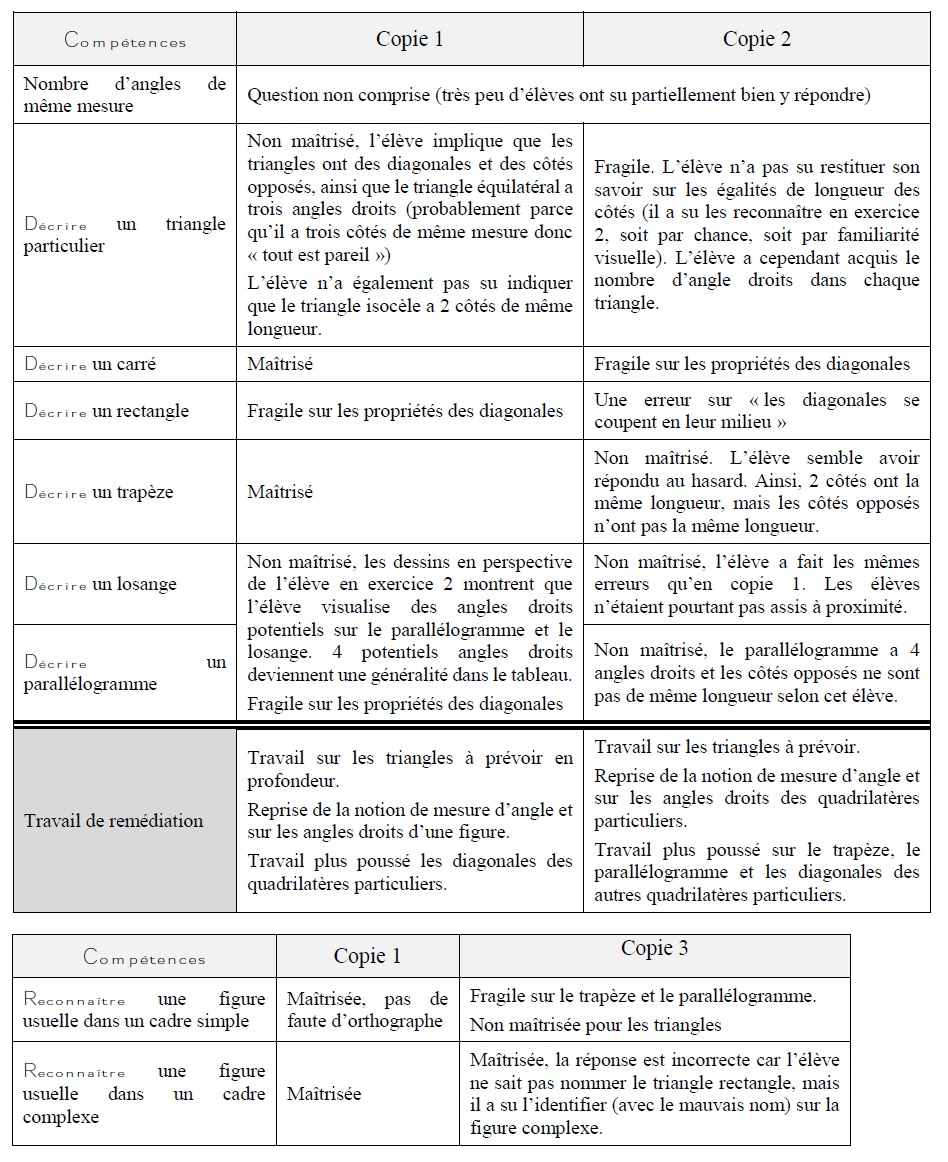
\includegraphics[scale=0.75]{img/Analyse_eval_diag_ju.jpg}
	\caption{Analyse des évaluations}
\end{figure}
\subsubsection*{Parcours différenciés}\label{parcours_diff3}
Le 3\up{e} parcours différencié sera plus détaillé à l'oral. Ci-dessous le parcours « triangles »\footnote{Les exercices sont ceux du manuel Transmath de 6\up{} (Nathan)}.
\begin{figure}[!h]
	\centering
	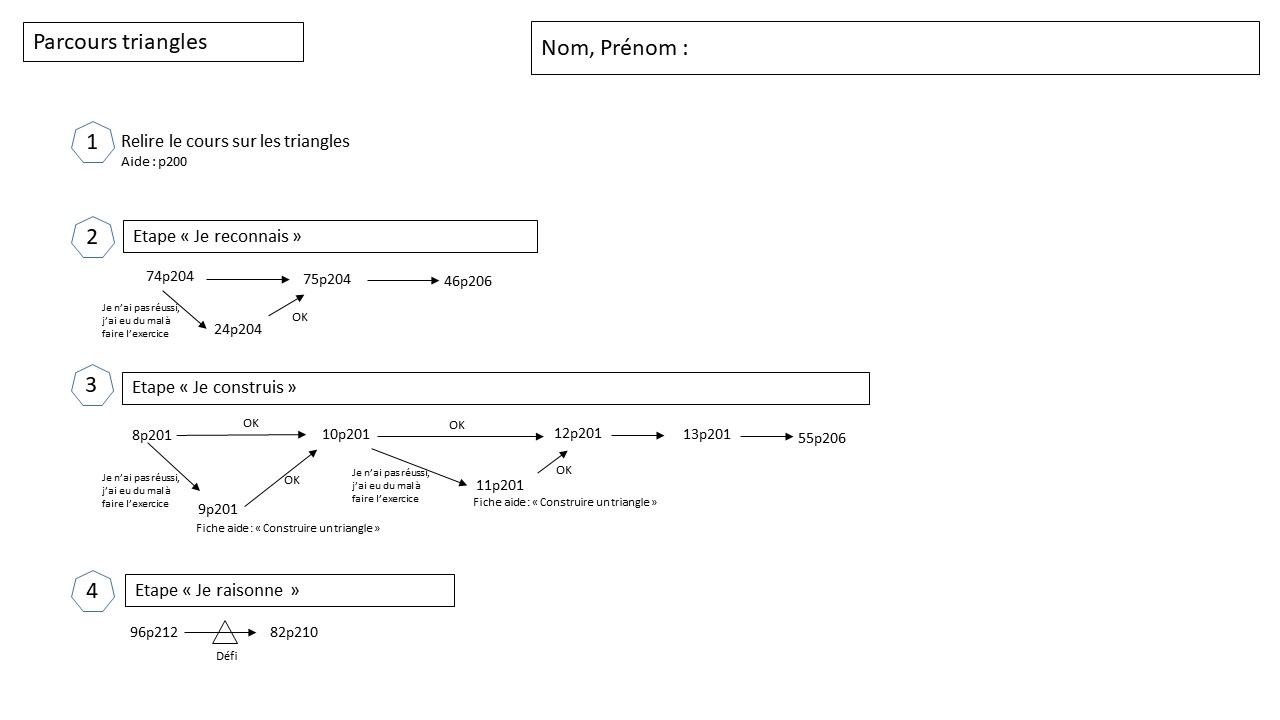
\includegraphics[scale=0.4]{img/parcours_triangles.jpg}
	\caption{Parcours triangle}
\end{figure}
\paragraph{}Tous les élèves effectuerons le parcours « \textit{3- Je construis} » car la classe de 6\up{e} est, selon moi, la classe où l'on peut le plus effectuer des constructions géométriques. Cette phase est effectuée lors d'une séance en demi-groupe.\\
Je distribuerai les parcours aux élèves en les dispensant de faire certains exercices (ou au contraire en leur demandant de commencer par l'exercice de remédiation).\\
Ainsi, parmi les élèves précédents, l'élève 1 commencera par l'exercice 24 p 204 puis il pourra effectuer l'exercice 74p204 (son parcours « \textit{Je reconnais} » sera une succession de flèches horizontales). L'élève 2 aura le parcours tel que présenté mais je lui demanderai de ne pas faire l'exercice "défi" tant qu'il n'aura pas terminé le parcours « \textit{Quadrilatères} ». L'élève 3 aura l'intégralité du parcours à effectuer, s'il est retard car il a passé beaucoup de temps sur le parcours « \textit{Quadrilatères} » par exemple, il n'aura pas à faire l'exercice 8 de l'étape « \textit{3- Je construis} ».
\paragraph{} Les exercices de l'étape « \textit{3- Je reconnais} » sont des exercices où les élèves doivent reconnaître les différentes représentations de triangles particuliers à l'aide de codages. Le parcours se termine par la reconnaissance des triangles au sein d'une figure complexe.\\
L'étape « \textit{3- Je construis} » comporte des programmes de constructions simple de triangles. En cas de non réussite de l'élève, celui-ci doit construire le même type de triangle mais à partir d'un croquis. Il aura ainsi un lien entre le programme de construction écrit, le croquis et la figure finale. Le parcours se termine sur une réflexion autour de la manière de construire une figure complexe composée de triangles et à partir d'un croquis. Cet exercice fait le lien avec le parcours suivant.\\
Dans « \textit{4- Je raisonne} », l'élève construit à partir d'un programme de construction, reconnaît les triangles particuliers à partir de leur définition et conjecture sur la nature des triangles au sein d'une figure complexe à l'aide de mesures effectuées. L'exercice défi demande une plus grande maîtrise de la langue française et des pratiques de raisonnement (« \textit{Sachant que...} », exercice avec aucune indication).
